% !TEX TS-program = pdflatex
% Compilation (pdflatex) : make (voir Makefile), c'est-a-dire
%   (les figures ps-files/*.pdf ont ete converties une fois pour toutes depuis
%    les .ps d'origine, avec 2 pt de marge autour de la boite englobante)
%   pdflatex LE2e ; musixflx LE2e ; makeindex LE2e ; pdflatex LE2e ; pdflatex LE2e
%\documentclass[12pt]{livre}
\documentclass[12pt]{book}
% Figures PostScript (ps-files/*.ps) : avec OzTeX, \special{epsf=...} ;
% ici graphicx. Avec pdflatex, epstopdf convertit chaque .ps en .pdf
% (une fois, avec repstopdf, autorise par defaut dans TeX Live).
\usepackage{graphicx}
\usepackage{epstopdf}
\epstopdfDeclareGraphicsRule{.ps}{pdf}{.pdf}{repstopdf #1 --outfile=\OutputFile}
\DeclareGraphicsExtensions{.pdf,.ps}
% Les trois macros d'origine, avec graphicx a la place du \special{epsf=...}
% d'OzTeX. Comme le \special, la figure ne prend aucune place : son coin
% inferieur gauche est au point courant et elle s'etend vers le haut et vers
% la droite ; le texte reserve la place (\vspace, \hspace) ou se superpose.
% En mode vertical, une boite de hauteur nulle (sans interligne) ; dans un
% paragraphe, une boite de taille nulle.
% ps-files/X.pdf (converti du .ps d'origine) a une marge de 2 pt autour de la
% boite englobante : on recule la figure d'autant (a l'echelle)
\newdimen\LEmarge 
\def\LEfigure#1#2{\LEmarge=#1\dimexpr 2pt\relax
  \kern-\LEmarge\raisebox{-\LEmarge}[0pt][0pt]{\includegraphics[scale=#1]{#2}}}
\newcommand\figurePS[2]{%
  \ifvmode
    {\dimen0=\prevdepth\nointerlineskip
     \vbox to 0pt{\vss\hbox to 0pt{\LEfigure{#1}{#2}\hss}}% 
     \prevdepth=\dimen0}%
  \else
    \smash{\rlap{\LEfigure{#1}{#2}}}%
  \fi}
%exemple: \includePostScript{MotifPavageQuadrilateres}{0.95}{0.95}
\def\includePostScript#1#2#3{\figurePS{#2}{{ps-files/#1}.pdf}}%
%exemple: \includevspacePostScript[6.5cm]{CroixDeCoins}{0.95}{0.95}
\def\includevspacePostScript[#1]#2#3#4{\vspace{#1}\includePostScript{#2}{#3}{#4}}
\def\includehvspacePostScript[#1,#2]#3#4#5{\vspace{#2}\centerline{\includePostScript{#3}{#4}{#5}\hspace{#1}}}
%
\usepackage[utf8]{inputenc}
\usepackage[T1]{fontenc}
\usepackage{latexsym} % \Box (fin des exemples)
\usepackage{musixtex}
\usepackage{comment}
%\usepackage[LY1]{fontenc}
%\usepackage{em}
\makeatletter
\renewcommand\@chapapp{}
\makeatother
% le paquet french (e-french) de 1999 casse les notes de bas de page
% avec le LaTeX actuel : babel en francais le remplace
\usepackage[french]{babel}
% legendes comme dans l'edition de 1999 (paquet french) : "Fig. 1.1 -- texte"
% en petites capitales, texte de la legende en italique
\makeatletter
\long\def\@makecaption#1#2{\vskip\abovecaptionskip
  \sbox\@tempboxa{#1~-- {\itshape #2}}%
  \ifdim\wd\@tempboxa>\hsize #1~-- {\itshape #2}\par
  \else\global\@minipagefalse\hb@xt@\hsize{\hfil\box\@tempboxa\hfil}\fi
  \vskip\belowcaptionskip}
% notes dans les boites (minipage) : lettre en exposant, comme en 1999
\AddToHook{env/minipage/begin}{\long\def\@makefntext#1{\parindent 1em
  \noindent\hb@xt@1.8em{\hss\@makefnmark}#1}}
\makeatother
% virgule decimale en mode math : 4,5 et non 4, 5
\DecimalMathComma
\addto\captionsfrench{\def\figurename{\textsc{Fig.}}\def\tablename{\textsc{Tab.}}}
% espacement des listes du paquet french (1999) : impose au debut de chaque
% liste, il l'emporte sur les reglages des listes du livre
\makeatletter
\let\LE@trivlist\@trivlist
\def\@trivlist{\setlength{\parsep}{0.2ex plus 0.1ex minus 0.1ex}%
  \setlength{\itemsep}{0.2ex plus 0.1ex minus 0.1ex}%
  \setlength{\topsep}{0.4ex plus 0.2ex minus 0.2ex}%
  \setlength{\partopsep}{1.6ex plus 0.8ex minus 0.8ex}%
  \LE@trivlist}
\makeatother
\usepackage{url}
\usepackage{xcolor}
\definecolor{darkblue}{HTML}{002AA3}%{002080}
\usepackage[colorlinks=true,hyperindex=true,hyperfigures=true,linktocpage=true]{hyperref}
\hypersetup{
    linkcolor=darkblue, % Color for internal links (sections, pages)
    citecolor=darkblue, % Color for bibliographical citations
    urlcolor=darkblue   % Color for external URLs
}
\def\chaptername{}

%%%%%%%%%%%%%%%%%%%%%%%%%%%
%%% NOUVELLES COMMANDES %%%
%%%%%%%%%%%%%%%%%%%%%%%%%%%

\input ROBOT12PT.tex                 % Robot souriant : \robot
\input ROBOTErreur12PT.tex           % Robot fache en cas d'erreur : 
                                     % \robotErr

\newcommand{\pascal}{\href{https://en.wikipedia.org/wiki/Pascal_(programming_language)}{\small \sc Pascal}}
\newcommand{\ocaml}{\href{https://en.wikipedia.org/wiki/OCaml}{OCaml}}
\newcommand{\python}{\href{https://en.wikipedia.org/wiki/Python_(programming_language)}{Python}}
\setlength{\emergencystretch}{2em} % messages du compilateur en \tt : longs mots insecables
\newcommand{\neglskip}{-2.5pt}       % diminution de l'espacement entre deux lignes de programme
\newcommand{\blk}{\hspace{0.7em}}    % taille d'un blanc en debut de ligne d'un programme

\newcommand{\parindentprog}{1.0em}   % identation des programmes
\newcommand{\carrenoir}{}            % pas de carre noir en marge de prgramme
%\newcommand{\mcl}{\small\bf}        % police des mots-cles
\font\mcl=cmbx10 scaled 1100
\newcommand{\cmt}{\footnotesize\tt}  % police des commentaires
%\newcommand{\idt}{\small\tt}        % police des identificateurs dans les programmes
\font\idt=ectt1000 scaled 1100   % T1 : lettres accentuees dans les programmes
\newcommand{\blc}{\small\tt}         % police des blancs de debut de ligne
\newcommand{\cha}{\small\tt}         % police des chaines de caracteres

\newcommand{\blanc}{\rule{0.1mm}{0.4ex}\rule{0.8em}{0.1mm}\rule{0.1mm}{0.4ex}}

\newcommand{\tiret}{\vspace{1.5mm}\noindent\rule{2mm}{0.25mm}\rule{2mm}{0mm}} % pour exos et corriges

\newcommand{\TITRE}{\rm PREMIÈRES LEÇONS DE PROGRAMMATION EN OCAML}
%\newcommand{\TITRE}{\rm LA PROGRAMMATION DES ORDINATEURS EXPLIQUÉE AUX ENFANTS}
%\newcommand{\TITRE}{\rm LA PROGRAMMATION DES ORDINATEURS EXPLIQUÉE PAR LE DESSIN}
%\newcommand{\TITRE}{\rm LA PROGRAMMATION EN PASCAL EXPLIQUÉE PAR LE DESSIN SUR ORDINATEUR}
\newcommand{\titre}{\sl Premières leçons de programmation en OCaml}
%\newcommand{\titre}{\sl La programmation des ordinateurs expliquée aux enfants}
%\newcommand{\titre}{\sl La programmation des ordinateurs expliquée par le dessin}
%\newcommand{\titre}{\sl La programmation en Pascal expliquée par le dessin sur ordinateur}


%%%%%%%%%%%%%%%%%%%%%%
%%% ENVIRONNEMENTS %%%
%%%%%%%%%%%%%%%%%%%%%%
\newtheorem{exemple}{Exemple}
\newtheorem{exercice}{Exercice}
\newtheorem{exercices}[exercice]{Exercice}
\newtheorem{corrige}{Corrigé}
\newtheorem{corriges}[corrige]{Corrigé}

%%%%%%%%%%%%%%%%%%%%
%%% MISE EN PAGE %%%
%%%%%%%%%%%%%%%%%%%%
%\headheight 16mm
%\headsep 10mm
%\textheight 192mm
%\textwidth 137mm
%\oddsidemargin 11.1mm
%\evensidemargin 11.1mm
% mesures de l'edition de 1999 : corps du texte 137 x 192 mm, en-tete 10 mm
% au-dessus ; pages impaires 26 mm a gauche (petit fond) et 12 mm a droite
\usepackage[paperwidth=175mm,paperheight=238mm,%
textwidth=137mm,textheight=192mm,%
inner=26mm,top=24mm,%
headheight=4mm,headsep=10mm,footskip=0pt,%
marginparwidth=0pt,marginparsep=0pt%
]{geometry}
\flushbottom
% make sure leading/trailing spaces work correctly in \verb
{\obeyspaces\gdef {\leavevmode\null\enskip\null}}

\makeindex

% Definition de la largeur du texte (\myparboxwidth) dans les
% addenda.
\newlength{\myparboxwidth}
\setlength{\myparboxwidth}{\textwidth}
\addtolength{\myparboxwidth}{-2em}

%%%%%%%%%%%%%%%%
% pages scannees de l'edition imprimee (couverture, pages de titre et de
% copyright au debut, page de l'imprimeur et 4e de couverture a la fin),
% tirees de CousotCousotCousotCousot1991.pdf ; recadrees sur la couverture
% et mises a l'echelle de la page, sans changer la numerotation du livre
\usepackage{pdfpages}
\newcounter{LEpage}
\newcommand\LEscans[1]{\setcounter{LEpage}{\value{page}}%
  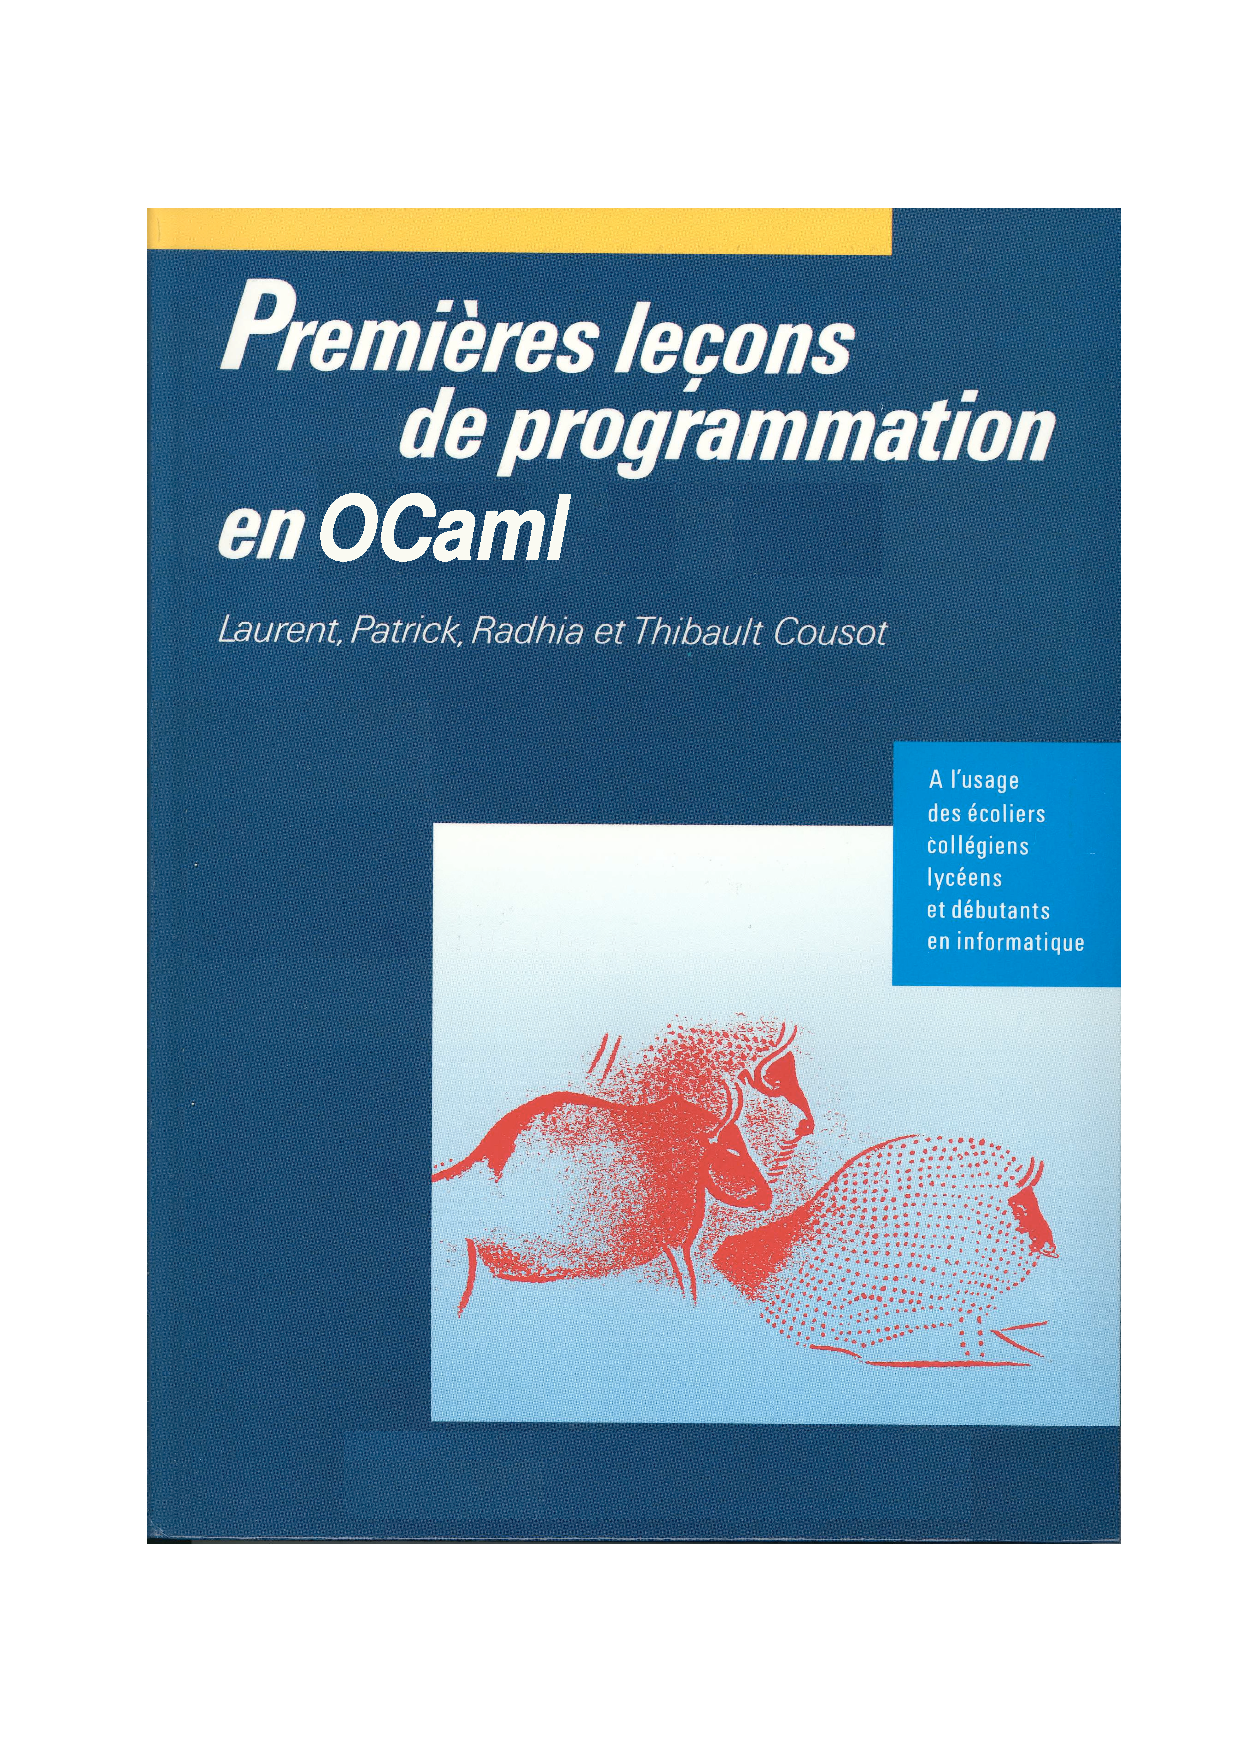
\includepdf[pages={#1},viewport=71 101 538 742,pagecommand={\thispagestyle{empty}}]{couvertures-aplaties.pdf}%
  \setcounter{page}{\value{LEpage}}}
\begin{document}
\LEscans{1-4}
%%%%%%%%%%%%%%%%
%\begin{comment}

%\tracingrestores=1

%%%%%%%%%%%%%
%%% TITRE %%%
%%%%%%%%%%%%%

\begin{titlepage}
\begin{centering}
\vspace{40mm}
\Huge\bf \TITRE\\
\vspace{15mm}
\Large\bf 
Laurent COUSOT \hspace{13mm} Patrick COUSOT\\
Radhia COUSOT \hspace{13mm} Thibault COUSOT\\
\vspace{15mm}
\large
\copyright\ \the\year\\
\end{centering}
\vspace{70mm}
\begin{quote}
\raggedleft\large
A l'usage des écoliers,\\
collégiens,\\
lycéens,\\
et débutants en informatique.
\end{quote}
\end{titlepage}

%%%%%%%%%%%%%%%%%%%%%%%%%%%%%%%%%%%%%%%%%%%%%
%%% TABLE OF CONTENTS AND LIST OF FIGURES %%%
%%%%%%%%%%%%%%%%%%%%%%%%%%%%%%%%%%%%%%%%%%%%%

\pagenumbering{roman}
\pagestyle{myheadings}
\markboth{\titre}{\sl Table des matières}
\thispagestyle{empty}
\makeatletter
\def\@starttoc#1{%
  \begingroup
    \makeatletter
    \thispagestyle{empty}
    \@input{\jobname.#1}%
    \if@filesw
      \expandafter\newwrite\csname tf@#1\endcsname
      \immediate\openout \csname tf@#1\endcsname \jobname.#1\relax
    \fi
    \@nobreakfalse
  \endgroup}
\renewcommand\tableofcontents{%
    \if@twocolumn
      \@restonecoltrue\onecolumn
    \else
      \@restonecolfalse
    \fi
    \chapter*{\contentsname
        \@mkboth{%
           \MakeUppercase\contentsname}{\MakeUppercase\contentsname}}%
    \@starttoc{toc}%
    \if@restonecol\twocolumn\fi
    }
\makeatother
\tableofcontents
\input AVERTISSEMENT.tex

%\markboth{\titre}{\sl Liste des figures}
%\thispagestyle{empty}
%\listoffigures

%\markboth{\titre}{\sl Liste des tables}
%\thispagestyle{empty}
%\listoftables

%%%%%%%%%%%%%
%%% LIVRE %%%
%%%%%%%%%%%%%

\chapter*{Introduction}
\pagenumbering{arabic}
%\label{ch:intro}
\markboth{\titre}{\sl Introduction}
\thispagestyle{empty}
\addcontentsline{toc}{chapter}{\protect \numberline{\ }Introduction}
\input INTRODUCTION.tex
\input REMERCIEMENTS.tex
\newpage
\thispagestyle{empty}

% Ch 1
\normalsize\rm
\chapter{Spécification}
%\label{ch:dessin}
\markboth{\titre}{\sl Spécification}
\thispagestyle{empty}
\input FAIRE-DES-DESSINS.tex

% Ch 2
{\normalsize\rm 
\chapter{Interaction}
%\label{ch:robot}  
\markboth{\titre}{\sl Interaction}
\thispagestyle{empty}
%%%% si l'on veut un robot Canvas (3x3) N, NE, E, SE, S, SW, W, NW
%%%%\input ROBOTPICT3x3.tex
%%%% si l'on veut un robot Canvas (2.46x2.46) N, NE, E, SE, S, SW, W, NW
\input ROBOTPICT2.46x2.46.tex
%%%% si l'on veut un robot picture LaTeX N, E, S, W
%%%%\input ROBOTPICTURES(4).tex
%%%% si l'on veut un robot picture LaTeX NE, SE, SW, NW
%%%%\input ROBOTPICTURES(8).tex
\input FAIRE-FAIRE-DES-DESSINS.tex
}

% Ch 3
\normalsize\rm 
\chapter{Programmation}
%\label{ch:prog-robot} 
\markboth{\titre}{\sl Programmation}
\thispagestyle{empty}
\input PROGRAMMER-LE-ROBOT.tex

% Ch 4
\normalsize\rm 
\chapter{Écriture, compilation et exécution de programmes}
%\label{ch:prog-pascal} 
\markboth{\titre}{\sl Écriture, compilation et exécution de programmes}
\thispagestyle{empty}
\input STRUCTURE-DES-PROGRAMMES.tex

% Ch 5
\normalsize\rm 
\chapter{Procédures}
\label{ch:proc-pascal} 
\markboth{\titre}{\sl Procédures}
\thispagestyle{empty}
\input PROCEDURES.tex

% Ch 6
\normalsize\rm 
\chapter{Sauts du robot au bord \protect\newline et au centre du cadre}
%\label{ch:ag-ad-eh-eb-ce} 
\markboth{\titre}{\sl Sauts du robot au bord et au centre du cadre}
\thispagestyle{empty}
\input ALLER-AU-BORD.tex

% Ch 7
\normalsize\rm 
\chapter{Boucles ``for''}
%\label{ch:for} 
\markboth{\titre}{\sl Boucles ``for''}
\thispagestyle{empty}
\input FOR.tex

% Ch 8
\normalsize\rm 
\chapter{Expressions entières}
%\label{ch:expr} 
\markboth{\titre}{\sl Expressions entières}
\thispagestyle{empty}
\input EXPR.tex

% Ch 9
\normalsize\rm 
\chapter{Appel de procédures \protect\newline avec paramètres}
\label{ch:appel} 
\markboth{\titre}{\sl Appel de procédures avec paramètres}
\thispagestyle{empty}
\input APPEL.tex

% Ch 10
\normalsize\rm 
\chapter{Grille de déplacement du robot}
%\label{ch:grille} 
\markboth{\titre}{\sl Grille de déplacement du robot}
\thispagestyle{empty}
\input GRILLE.tex

% Ch 11
\normalsize\rm 
\chapter{Constantes}
%\label{ch:const} 
\markboth{\titre}{\sl Constantes}
\thispagestyle{empty}
\input CONST.tex

% Ch 12
\normalsize\rm 
\chapter{Peinture}
\label{ch:peinture}
\markboth{\titre}{\sl Peinture}
\thispagestyle{empty}
\input COULEUR.tex

%Ch 13
\normalsize\rm 
\chapter{Déclarations de procédures avec paramètres}
%\label{ch:declproc} 
\markboth{\titre}{\sl Déclarations de procédures avec paramètres}
\thispagestyle{empty}
\input DECLPROC.tex

% Ch 14
\normalsize\rm 
\chapter{Repère cartésien}
%\label{ch:repcar} 
\markboth{\titre}{\sl Repère cartésien}
\thispagestyle{empty}
\input REPERE.tex

% Ch 15
\normalsize\rm 
\chapter{Test ``if''}
%\label{ch:if} 
\markboth{\titre}{\sl Test ``if''}
\thispagestyle{empty}
\input IF.tex

%Ch 16
\normalsize\rm 
\chapter{Expressions booléennes}
%\label{ch:bool} 
\markboth{\titre}{\sl Expressions booléennes}
\thispagestyle{empty}
\input BOOL.tex

% Ch 17
\normalsize\rm 
\chapter{Boucles ``while''}
%\label{ch:while} 
\markboth{\titre}{\sl Boucles ``while''}
\thispagestyle{empty}
\input WHILE.tex

% Ch 18
\normalsize\rm 
\chapter{Codage}
%\label{ch:codage} 
\markboth{\titre}{\sl Codage}
\thispagestyle{empty}
\input CODAGE.tex

% Ch 19
\normalsize\rm 
\chapter{Expressions rationnelles}
%\label{ch:real} 
\markboth{\titre}{\sl Expressions rationnelles}
\thispagestyle{empty}
\input REAL.tex

% Ch 20
\normalsize\rm 
\chapter{Rotations et translations}
%\label{ch:angles} 
\markboth{\titre}{\sl Rotations et translations}
\thispagestyle{empty}
\input ANGLES.tex

% Ch 21
\normalsize\rm 
\chapter{Récursivité}
\label{ch:rec} 
\markboth{\titre}{\sl Récursivité}
\thispagestyle{empty}
\input RECURSIVITE.tex

% Ch 22
\normalsize\rm 
\chapter{Variables}
%\label{ch:var} 
\markboth{\titre}{\sl Variables}
\thispagestyle{empty}
\input VAR.tex
\clearpage

\normalsize\rm 
\markboth{\titre}{\sl Bibliographie}
\addcontentsline{toc}{chapter}{\protect \numberline{\ }Bibliographie}
\label{ch:biblio} 
\thispagestyle{empty}
\input BIBLIOGRAPHIE.tex

%\end{comment}
%Appendix
{
% Definition de la taille du texte dans l'appendix
\newcommand{\apxFontSize}{\small}
%
\normalsize\rm 
\chapter*{Résumé des commandes \protect\newline du robot}
% pages du resume non etirees (\flushbottom ecartait le texte du titre et
% les tableaux entre eux)
\raggedbottom
\addcontentsline{toc}{chapter}{\protect \numberline{\ }Résumé des commandes du robot}
%\label{ch:cmd} 
\markboth{\titre}{\sl Résumé des commandes du \protect\robot}
\thispagestyle{empty}
\input CMDrobot.tex %resume des commandes du robot
}

\newpage                 % sauter un page paire page blanche
\flushbottom
\thispagestyle{empty}    %
\ \\                     %
\ \\                     %
\newpage                 % 
\thispagestyle{empty}    %

\markboth{\titre}{\sl Index}
\thispagestyle{empty}
\addcontentsline{toc}{chapter}{\protect \numberline{\ }Index}
% la 1re page de l'index (\thispagestyle{plain} de theindex) sans numero en
% bas de page : footskip est nul, le numero chevauchait la derniere ligne
\makeatletter\let\ps@plain\ps@empty\makeatother
\input{\jobname.ind}

% Bon de commande des disquettes de l'edition Pascal : sans objet pour OCaml
%\thispagestyle{empty}
%\addcontentsline{toc}{chapter}{\protect \numberline{\ }Bon de commande}
%\input BONdeCOMMANDE.tex

%\typeout{***}
%\typeout{*** Dans \jobname.toc :}
%\typeout{*** 1 - Ajouter une premiere ligne : \protect\thispagestyle{empty}}
%\typeout{*** 2 - Enlever les \protect\newline}
%\typeout{***}

% page 5 des scans (mentions de l'imprimerie Louis-Jean, 1991) remplacee
% par une page blanche pour garder la 4e de couverture en page paire
\LEscans{{},6}
\end{document}
